% use pdfLaTeX!!!
\pdfoutput=1
\documentclass[10pt]{article}

\usepackage{naacl2021}			% Style and Formatting for Camera-Ready PDF
\usepackage{times}				% standard
\usepackage{latexsym}			% standard
\usepackage[T1]{fontenc}		% proper rendering and hyphenation of words containing Latin characters 
\usepackage[utf8]{inputenc}		% files encoded as UTF8
\usepackage{microtype}			% improve layout and save space

%%%%%%%%%%%%% BEGIN ADDED PACKAGES %%%%%%%%%%%%%%%%%%%%%
% Text
\usepackage{comment}
\usepackage{enumitem}
\setlist[itemize]{noitemsep, topsep=0pt, parsep=0pt}

% Tables
\usepackage{booktabs}
\usepackage{float}
\restylefloat{table}

% Graphics
\usepackage{graphicx}           % images
\usepackage{caption}			% to include subfigures
\usepackage{subcaption}

% Subject specific 

% Formatting
\usepackage{placeins}
\usepackage{hyperref}           % clickable links in the document (should be last package!)

%%%%%%%%%%%% END ADDED PACKAGES %%%%%%%%%%%%%%%%%%%%%%

\title{Lab Course "Ethical AI": Explaining Discrimination with Data from the European Social Survey}

% For several authors from the same institution:
\author{Leo Holzhauer \and Annalena Kofler \and Christopher Sendlinger\\
	\texttt{firstname.lastname@tum.de}\\
	Technical University Munich}

\begin{document}
	\maketitle
	\pagenumbering{roman}
	
	\begin{abstract} % Anna
		Discrimination and its versatile forms have sparked a significant public interest in the recent years. As various social factors influence the subjective feeling of being discriminated against, the question arises whether discrimination can be predicted using Machine Learning approaches.  
		Our work for this project is based on the data set of the European Social survey conducted in 2018-2020 and is consisting of	49,000 participants. After establishing a data preparation pipeline, we utilized unsupervised methods to find general patterns in the data which turned out to be not related to discrimination. To predict discrimination directly, we compared different supervised models like decision trees, random forests with boosting, Support Vector Machines, logistic regression, and neural networks. Multiple approaches for feature sub-selection and adjusting the imbalanced classes were considered. XGBoost with all features and weighted classes performed best on the F1 score. It was possible to find and explain contributing variables to discrimination and understand false predictions with SHAP and cosine similarity. 
	\end{abstract}
	
	\section{Introduction} % Leo
	With the recent rapid advancements in applications for Artificial Intelligence (AI), concerns for the ethical use of these applications are growing simultaneously. Security features to ensure privacy and fairness of AI applications as well as AI applications in a technical field with direct ethical considerations, such as fake image detection, are being researched and developed. However, little emphasis has been put on explaining predictions and on the application area of social sciences \citep{grimmer:2021}.
	
	In the social sciences, data is primarily used to model and understand social structures \citep{grimmer:2021}. This way, non-beneficial conditions, and processes become visible, which have the potential to cause social grievances or distress and suffering for the individuals involved. An improved understanding of the influential factors enables the development of efficient intervention responses and therefore offers a promising use case for a way to apply AI in an ethical relevant and significant way. An example for a non-beneficial condition is the social exclusion based on unemployment, which was modeled with various Machine Learning (ML) methods from \citep{serrano:2019-2}. With the developed application social workers in Northern Spain were supported in an efficient use of their limited temporal capacities to search for socially excluded individuals.
	
	In this work, a similar approach was used to model the social structures involved in another condition which implies individual suffering: the self-reported experienced discrimination of individuals. After an initial data investigation and preparation, unsupervised as well as supervised ML methods were used to find factors most influential for the perceived feeling of being discriminated against.
	
	However, it has to be considered that feeling discriminated against is a subjective opinion that depends on a multitude of different social factors. Firstly, the participant has to be informed and educated about the meaning of discrimination and its different forms. Secondly, the person has to be able to understand and conclude whether they are discriminated against. Thirdly, the participant has to be willing to share this sensitive and personal information in a face-to-face conversation with the interviewer. As a result, the possibility of answers not reflecting the true feeling of the respondent to this question has to be taken into account during evaluation. Therefore, an analysis to better explain model performance deviations and similar data points with different target values was done. 
	
	
	\section{Data Investigation} % Anna
	\subsection{Data Set} \label{sec:data_set}
	This project is based on the data collected in round 9 of the European Social Survey (ESS) which is an academically-driven project conducted every two years in 38 countries up to date. The general goal of the survey is the monitoring and evaluation of public attitudes and values.
	The chosen data set (ESS9-2018 \citep{ESS9:2021}) was acquired in the years 2018-2020 and contains data from at that time 25 European and six non-European countries. The full list of countries can be found in Appendix \ref{sec:participating_countries}. The participants were selected via random stratified sampling methods. To ensure a high response rate, the participants were called or visited up to eight times and participation benefits such as vouchers were offered in some countries. The conducted face-to-face interview had a duration of approximately one hour and contained 512 questions in different categories. The names of the categories and illustrative examples for questions can be found in Table \ref{tab:ess9_categories} in the appendix \cite{ESS9_data_documentation:2021}. 
	
	Since a high dimensional feature space with a limited number of data points can propose challenges for a ML algorithm, we decided to manually reduce the number of questions from 529 to 113 with a focus on potential indicators for discrimination. A clear choice for a feature to include was for example "Belong to minority ethnic group", while a clear choice to leave it out was "Interview length in minutes". If a question received more invalid than valid answers, it was not included in further analysis.
	The answers to the survey questions are based on different scales such as categorical or numerical, dependent on the type of the question. For example questions like "How religious are you?" could be answered with an integer value from 0 ("Not religious at all") to 10 ("Very religious"), while a question asking for the annual net pay could be answered with any numerical value. For each question there were the options "Refusal", "Don't know", and "No answer" that were encoded as outlier values in the data set. As an example, outliers were encoded with 77, 88, 99 for the question "How religious are you?".
	
	The target variable we tried to learn and predict is formulated as "Would you describe yourself as being a member of a group that is discriminated against in this country?". 
	If this question was answered with "Yes", it was possible to select the specific form of discrimination. Since the subcategories contained less than 1000 data points each (see Appendix \ref{sec:target_variable}), we decided to focus on the binary variable of discrimination. A total of 3,593 participants referred to themselves as being discriminated against, while 43,062 people do not feel discriminated. An illustration of this distribution can be found in Figure \ref{fig:discriminated_dist}. The fact that the data distribution is imbalanced has to be taken into account in the data preparation for the ML approaches. 
	When the number of discriminated people is normalized by the number of participants per country, it can be observed that some countries have a high percentage of people feeling discriminated (c.f. Figure \ref{fig:discriminated_country}). These countries are Iceland, the United Kingdom, France, and Montenegro which can be explained with the dominating subcategories in the specific country (see Appendix \ref{sec:target_variable}). 
	\begin{figure}[h]
		\centering
		\includegraphics[width=0.4\textwidth]{../figures/tex/discriminated_country}
		\caption{Percentage of participants per country that describe themselves as being discriminated against.}
		\label{fig:discriminated_country} % Maybe move to appendix
	\end{figure}
	
	\subsection{Correlation of Variables} % Leo
	A variant to determine linear dependencies between feature $x$ and target $y$ is the Pearson Correlation coefficient (PCC). A value of $+1$ corresponds to a strong linear proportionality between $x$ and $y$, whereas a value of $-1$ corresponds to a strong inverse linear proportionality. With a value of $0$ it can be said with certainty that there is no linear relation between $x$ and $y$.
	
	We calculated the PCC for all preselected features. The overall tendency is that the linear correlations within the data set are low, which is described in detail in Appendix \ref{sec:pcc}. In particular, the correlations with all other features and the target variable "Member of group discriminated against in this country" are below an absolute value of $0.25$, which can be considered a weak linear correlation. Nevertheless, when sorted by magnitude, the resulting order of features leaves room for reasonable conclusions, as can be observed in Figure \ref{fig:pcc_targets}. 
	
	\begin{figure}[h]
		\centering
		\includegraphics[width=0.4\textwidth]{../figures/tex/pcc_targets_15}
		\caption{Pearson Correlation coefficients for "Member of group discriminated against in this country" (strongest 15, sorted by magnitude).}
		\label{fig:pcc_targets} % Maybe move to appendix, enlarge handles
	\end{figure}
	
	Put into perspective, the relatively high correlations of the features "Trust in the police", "Hampered in daily activities by illness/disability/infirmity/mental problem" as well as "Belong to minority ethnic group in country" w.r.t. the target are likely to mirror an existing correlation observed by individuals experiencing discrimination because of their ethnicity or disability. However, this mere quantitative analysis alone is not enough but rather intends to serve as a guideline for setting priorities for a further qualitative investigation based on expert knowledge from the field of the social sciences. 
	In this work, we used the results of the correlation analysis as a selection criterion to reduce the number of inputs for the supervised ML models. The resulting subset was part of an additional evaluation dimension, further described in Subsection \ref{ssec:features}.
	
	
	\section{Data Preparation}
	A general overview of the necessary steps for the preparation of the data is highlighted with blue color in Figure \ref{fig:data_pipeline}.
	\begin{figure*}[h]
		\centering
		\includegraphics[width=0.85\textwidth]{../figures/tex/data_pipeline}
		\caption{Data pipeline for supervised approaches.}
		\label{fig:data_pipeline}
	\end{figure*}
	This process contains preprocessing steps followed by different options for the selection of features. These options were evaluated separately to determine whether a subset of the questions resulted in an improved performance of the ML algorithm. For supervised learning, the data was split into a training and test set. On the training set, we experimented with different sampling techniques with the goal of increasing the performance.
	
	\subsection{Preprocessing}
	In order to prepare the data for the different ML procedures, it was necessary to encode outliers, exclude NaN values, and represent the unordered, categorical variable "country" using one-hot encoding. This way, the number of data points was reduced from 49519 to 46655 and the number of features increased from 113 to 139. For more detailed information, the interested reader may refer to Appendix \ref{sec:details_preprocessing}.
	
	\subsection{Feature Selection} % Leo
	\label{ssec:features}
	We integrated feature selection into the data preparation pipeline to evaluate the influence of different feature sets on the performance of the ML models, this way aiming on drawing further conclusions on the inter-dependencies within the data set. A better model performance based on a specific feature set may indicate higher correlations with the target of the features within this set, therefore enabling a deeper understanding of the importance of factors influencing the perception of discrimination.
	From the already manually selected and preprocessed 139 features, we extracted three additional subsets of these features. Firstly, the 30 features having the strongest linear correlation with the target according to the PCC values. Secondly, a subset based on iterative queries to the GPT-3 davinci model of OpenAI \cite{brown:2020}. To generate this subset, we stated a prompt to the model containing all of the feature definitions and the question to extract the ten most influential ones w.r.t. the target. This procedure was repeated ten times, the results were listed and sorted in descending order according to their number of appearances in the answers. This way, another subset with 30 features was generated. This subset had also the purpose to test the assumption of whether or not there is already implicit knowledge about the influential factors on discrimination in the training data of GPT-3. Thirdly, all of the features within the ESS category "Human values" were used to form the last subset. 
	
	\subsection{Splitting} 
	The data set was split into a training and test set in a ratio of 90/10. From the training data set, a validation data set was separated for hyperparameter optimization when needed. The remaining training data was used to learn the model parameters.
	
	\subsection{Sampling}\label{sec:sampling}
	As imbalanced distributions of the target variable are a well-known problem in the ML community \cite{chawla:2002, he:2008}, we expected challenges in the supervised learning approaches. To mitigate such problems, we investigated the performance of different sampling methods. As a baseline, we trained the different ML methods using the original data set which will be called "no sampling" in the following. Additionally, over- and undersampling can be utilized to engineer a data set with balanced class labels. In undersampling, the number of data points in the majority class is reduced randomly until it is equal to the minority class. In oversampling, new data instances of the minority class are generated artificially via discrete interpolation between minority data points until the classes are balanced. Here, we used the method SMOTEN \cite{chawla:2002}. 
	Furthermore, it is possible to assign weights to each data point that inform the model of the importance of a specific data point. The weights were chosen as the ratio of elements in the minority over the majority class. In the following, we refer to this method as "weighting".
	
	\section{Unsupervised Learning}
	\subsection{Principal Component Analysis (PCA)} % Chris, Anna
	Including the one-hot encoded country information, the data is located in a 139-dimensional feature space. To reduce the number of features, one can use methods like Principal Component Analysis (PCA). For visualization purposes, a target dimension of $k=2$ is common.
	Only PCC as feature selection gave visual distinct structures, pictured in Figure \ref{fig:pca}. The other selections formed uninformative big clouds of all data samples.
	Principle component analysis leads to the fact that the y-component is mostly defined by three features (mother/father/self born in the country), which can be interpreted as the heritage of a person.
	Red data points correspond to participants where neither they, nor their parents are born in this country, while dark blue values represent participants where they and their parents are born in this country.
	Unfortunately, the dimensional reduction does not carry any information about our target variable which can be seen in Figure \ref{fig:pca}. Nevertheless, this shows that there are underlying structures in our data that can be used for our classification task.
	\begin{figure}
		\centering
		\includegraphics[width=0.23\textwidth]{../figures/tex/pca_cntry}
		\includegraphics[width=0.23\textwidth]{../figures/tex/pca_discr}
		\caption{PCA (k=2), coloring based on persons heritage (left) / target variable (right)}
		\label{fig:pca}
	\end{figure}
	
	\subsection{K-Means Clustering} % Chris
	Building upon the results of dimensionality reduction, the next step was to identify clusters in the data. The simplest method to use here is K-Means, which builds $K$ groups of similar data points. Our goal was again to differentiate between the participants based on the different answers they gave to the target question. The results on the reduced data using PCA ($k = 2$) however were not promising, which can be seen in Figure \ref{fig:pca}. No clear distinctions between the different answers to the target question can be made.
	
	\subsection{Hierarchical Clustering} % Chris
	Hierarchical clustering builds up clusters based on the similarity between different objects in the data set. Unlike K-means, it can provide insight into the composition of clusters, which may be helpful for our task. Also, this method can not find clusters that separate our target, reasons for that are described in the following subsection.
	
	\begin{comment}
		\begin{figure}[h] 
			\centering
			\includegraphics[width=0.45\textwidth]{../figures/tex/hier_clustering}
			\caption{Dendrogram for the hierarchical clustering}
			\label{fig:hier_clustering} % put into Appendix or remove completely (depending on the size of the Appendix xD)
		\end{figure}
	\end{comment}
	
	\subsection{Conclusion}
	The tested unsupervised methods are not promising for our data and the question we want to answer, which has multiple reasons.
	The first problem was that the high dimensionality lies within the nature of our data set. To address this, standard approaches like PCA were used to reduce the dimensions with low variance and give the clustering methods a better chance to find structures within. On our data, this led to point clouds where both target classes are indistinguishable and mixed up.
	Arising from this is the second problem, the used clustering methods can not identify meaningful clusters for the given question. This problem is again rooted in the data since the difference between a discriminated and a not discriminated participant often lies in very small details and not fundamentally different beliefs. This fine contrast can not be picked up by the used methods.
	
	\section{Supervised Methods} % Anna
	Although no general structure was found in the data, supervised learning techniques can be employed to predict the feeling of discrimination of individual participants. Different supervised algorithms have proven successful in the context of predicting environmental attitudes and beliefs based on ESS8 data \citep{yektansani:2021}. These models are: random forest, logistic  regression, and neural networks. In addition to these algorithms, we experimented with decision trees and Support Vector Machines (SVM). For the random forest with boosting, we specifically used the XGBoost classifier.
	
	The F1 score and the weighted F1 score were investigated as evaluation metrics for the model performance. The weighted F1 score calculates the mean of the F1 scores of the individual classes while considering the actual occurrences in the data set. Therefore, it is specifically designed for imbalanced data sets and shows good overall values for all investigated models (c.f. Figure 			\ref{fig:f1_weighted}). However, we observed an undesirably large value of False Positive instances in the confusion matrices. The reason for this is that the weighted F1 score assigns greater contribution to the class with more examples in the data set. In our case, we observed a larger number of discriminated people being labeled as not discriminated. Since our focus lied on the 		accurate prediction of truly discriminated people, we decided to use the normal F1 score to prevent a large influence of not discriminated participants. The unweighted F1 score has the best trade-off between correctly identifying the most discriminated people and keeping the wrong identifications of not discriminated participants moderately low. The best hyperparameters for each model were optimized using the F1 score. 
	
	\subsection{Decision Tree} % Leo
	Providing the least complex ML architecture from the mentioned methods, decision trees are the most promising when it comes to explainability and inferring knowledge about the dependencies of model input and output. An example to exploit the explaining qualities of the decision trees can be found in Appendix \ref{ssec:dt}. The used hyperparameters are: min\textunderscore samples\textunderscore leaf:$0.001$, max\textunderscore depth: $\left\{3, 99\right\}$. The best performing model evaluated uses feature set "dvc" and method "wgh".
	
	\subsection{XGBClassifier} % Chris
	XGBoost \cite{Chen:2016:XST:2939672.2939785} implements ML algorithms using gradient boosting. The XGBClassifier combines the predictive power of decision trees with gradient boosting, which usually outperforms random forests. The used hyperparameters are: Booster: gbtree, max\textunderscore depth:$10$, learning\textunderscore rate:$0.1$, n\textunderscore estimators:$125$. The best performing model evaluated uses feature set "all" and method "wgh".
	
	\subsection{Support Vector Machines (SVM)} % Chris
	Support Vector Machines (SVM) \cite{cortes1995support} try to find a decision boundary between the different classes of the data set. The used hyperparameters are: loss: hinge, penalty: elasticnet. The best performing model evaluated uses feature set "all" and method "wgh".
	
	\subsection{Logistic Regression} % Anna 
	While SVMs try to maximize the margin among class variables, logistic regression aims at maximizing the conditional likelihood of the data. Although the approaches are similar, one might outperform the other dependent on the data.
	The optimized hyperparameters for logistic regression are the solver (newton-cg, lbfgs, sag, saga), the regularization type (none, $L_1$, $L_2$) with the inverse regularization strength $C$, as well as the tolerance for stopping. The best performing model used the solver saga, $L_2$ regularization with $C=0.1$, and a tolerance of $0.001$.
	
	\subsection{Neural Network (NN)} % Anna
	Investigations regarding the application of deep neural networks (NNs) to social science data have shown that small NNs with a few hidden layers and a limited number of neurons per layer perform best \cite{serrano:2019}. Similarly to this research, we chose small architectures for hyperparameter tuning which included networks with one hidden layer and 20, 50, or 100 neurons as well as two or three hidden layers where the number of neurons depended on the number of inputs $(N_{\mathrm{in}}, 0.5 \cdot N_{\mathrm{in}} ), (N_{\mathrm{in}}, 0.5 \cdot N_{\mathrm{in}}, 0.2 \cdot N_{\mathrm{in}})$. Furthermore, we included the activation functions ReLU, tanh, and Sigmoid in the hyperparameter search. The following hyperparameters were fixed due to computational limitations: optimizer Adam, a constant learning rate of $0.001$, batch size of 200, and a stopping tolerance of $0.001$. The best performing model has ReLU as the activation function and a single hidden layer with 20 neurons.
	Since the MLPClassifier class of sklearn does not support weighting, those values are set to zero in Figures \ref{fig:f1} and \ref{fig:f1_weighted}.
	
	\subsection{Best Model} % Anna und Chris
	The overall best model regarding the unweighted F1 score, is the XGBClassifier using the feature set "all" and weighting of the classes (c.f. Figure \ref{fig:cf_matrix}) .
	The unweighted F1 score of $0.362$ and a precision of $0.254$ make it the most predictive model that was trained. Considering the highly unbalanced data set and the inherently difficult target, this result is good. 
	
	\begin{figure}
		\centering
		\includegraphics[width=0.45\textwidth]{../figures/tex/cf_matrix}
		\caption{Confusion matrix for the best model. Total numbers for True/False Positive/Negative and number of explainable False Positive/Negative in the test set}
		\label{fig:cf_matrix}
	\end{figure}
	\begin{figure*}
		\centering
		\begin{subfigure}[t]{\textwidth}
			\includegraphics[width=\textwidth]{../figures/tex/f1score_weighted}
			\caption{Weighted F1 scores}
			\label{fig:f1_weighted}
		\end{subfigure}
		\begin{subfigure}[t]{\textwidth}
			\includegraphics[width=\textwidth]{../figures/tex/f1score}
			\caption{F1 scores}
			\label{fig:f1}
		\end{subfigure}
		\caption{Overview of metrices for all supervised methods (decision tree, XGBoost, SVM, logistic regression, small NN), dependent on the chosen feature selection method (columns) and sampling method (rows). The abbreviations can be found in Table \ref{tab:abbreviations}.}
	\end{figure*}
	
	\section{Explainability} % Chris
	To understand the predictive power and decision-making process of the model, different analyzing methods are used and combined. 
	\subsection{SHAP}
	Shapley Additive Explanations (SHAP) \cite{NIPS2017_7062} is a game theoretic approach to explaining the output of ML models. It can give insight into the impact of different input features on the output classification of the model. Figure \ref{fig:summary_plot} shows a summary plot for our best XGBClassifier; positive SHAP values are contributing towards classifying a person as discriminated while negative have the opposite effect. The coloring indicates what values of the feature generate the given SHAP value. The feature "Belong to minority group" (blgetmg) with the answer "No" (Value 2, Red) counteracts discrimination, while answer "Yes" (Value 1, Blue) is a strong indicator for it. Every feature can be analyzed in this way giving a good overview of high-risk characteristics.
	\begin{figure}[h]
		\centering
		\includegraphics[width=0.45\textwidth]{../figures/tex/summary_plot}
		\caption{SHAP summary plot: Positive SHAP values are contributing towards classifying a person as discriminated while negative ones have the opposite effect. The coloring indicates what values of the feature generate the given SHAP value. For abbreviations see Table \ref{tab:abbreviations}}
		\label{fig:summary_plot}
	\end{figure}
	
	\subsection{Cosine Similarity}
	Cosine similarity allows us to calculate a value in the range $[-1,1]$ that describes how similar two vectors are, with the maximum being identical to one another and the minimum being the exact opposite of each other. Analyzing the predictive power of our model using this method yields an explanation of why the model falsely classifies some samples. If we can find True Positives/Negatives for our wrongly classified False Positives/Negatives with a high similarity score, we can infer that our model made that mistake based on the subjectivity of the target variable.
	Using a threshold of 0.9 for the described similarity score, 65 of 131 participants, which answered that they feel discriminated against but our model predicted that they are not discriminated against (False Negative), can be explained by other similar persons that are True Negatives.
	307 of 671 False Positives can be explained by an equivalent in the True Positives. (Figure \ref{fig:cf_matrix})
	Again, this shows the underlying problem for the target variable, discrimination, is a very subjective topic. Persons that are very similar regarding the survey answers can have very different feelings and understandings of discrimination.
	
	\subsection{Selected Example} % Chris
	Using the explained similarity method and the SHAP values False Positives/Negatives become explainable. To illustrate this, a False Positive is compared with its corresponding similar True Positive (>0.999). Figure \ref{fig:ex_dscr} shows person \#2843 (TP) and Figure \ref{fig:ex_not_dscr} shows person \#1830 (FP). Most descriptive similarities: Both are living in Italy; neither they nor their parents were born there; both are in their early thirties. Their only crucial difference is that person \#2843 belongs to a minority group and the other has not answered this question. Because of these similarities in the most important features regarding discrimination, the model misclassified the second person.
	\begin{figure*}
		\centering
		\begin{subfigure}[t]{\textwidth}
			\centering
			\includegraphics[width=\textwidth]{../figures/tex/ex_dscr}
			\caption{Person \#2843 classified as True Positive.}
			\label{fig:ex_dscr}
		\end{subfigure}
		\begin{subfigure}[t]{\textwidth}
			\centering
			\includegraphics[width=0.99\textwidth]{../figures/tex/ex_not_dscr}
			\caption{Person \#1830 classified as False Positive.}
			\label{fig:ex_not_dscr}
		\end{subfigure}
		\caption{Comparison of the most influential SHAP values and their impact on the prediction of a True Positive and a False Positive.}
	\end{figure*}
	
	\section{Conclusion and Outlook} % Leo
	
	The explainability results allow us to understand why the unsupervised methods failed on our classification task. Two very similar persons can answer differently on whether or not they feel discriminated against. The differences lie within small deviations
	and not fundamentally different lifestyles or circumstances, which could be identified using the survey data. 
	
	Overall, no relevant clusters were found in unsupervised methods based on discrimination. However, statistical analysis and explainability of supervised methods yielded promising and interpretable results. Based on the findings, certain features are very likely to be good indicators for discrimination, e.g. "Belong to minority ethnic group" or "Hampered in daily activities by illness/disability/infirmity/mental problem". 
	
	Limitations were encountered during the elaboration of this work. On the one hand, discrimination is overall challenging to predict due to similar answers of participants, the imbalanced data set, and a used average over various heterogeneous European countries. On the other hand, discrimination is inherently a difficult target. Since it is a self-reported value, knowledge about discrimination is required to access it as well as a sensitization. Furthermore, it is influenced by many factors, e.g. potentially different definitions of discrimination dependent on the country or the individuals social environment.
	
	Further qualitative investigation incorporating expert knowledge from the social sciences is required to evaluate the validity of the correlations and similarities found. Additionally, a differentiation w.r.t. the multitude of reasons for discrimination might be promising for improved insights into the model dependencies. However, these improvements are currently limited by the small amount of positive target values and only feasible if the amount of data points per ESS cohort will improve significantly in the future. 
	
	\begin{comment}
		\begin{itemize}
			\item explainability allows us to explain why the unsupervised methods failed (due to similar examples in both classes) % Chris
			\item all, not only some FP/FN have to be analyzed
			\item formulate conclusion from poster
		\end{itemize}
	\end{comment}
	
	\section*{Acknowledgments}
	We would like to thank Tobias Eder for his supervision, advice, and ideas regarding our project. The bi-weekly discussion sessions were very helpful, interesting, and a lot of fun.
	
	
	\bibliographystyle{acl_natbib}
	\bibliography{custom}
	
	
	\appendix
	\section{Appendix} \label{sec:appendix}
	
	\begin{table*}[h!]
		\centering
		\begin{tabular}{@{}ll@{}}
			\toprule
			Category & Example questions\\ \midrule
			Media and social trust & Time in minutes spent on consuming news per day\\ 
			Politics & Signed petition in last 12 months\\ 
			Subjective well-being, social exclusion, health, & Subjective happiness, Parents born in this country\\ religion, national and ethnic identity &  \\ 
			Timing of life & Ever given birth to/fathered a child\\ 
			Socio-demographics & Level of education\\ 
			Justice and fairness & Decisions in country politics are transparent\\
			Human values & Important to care for others \\ \bottomrule
		\end{tabular}
		\caption{Categories and exemplary questions of ESS9 data set \cite{ESS9_data_documentation:2021}.}
		\label{tab:ess9_categories}
	\end{table*}
	
	\begin{table*}[h!]
		\centering
		\begin{tabular}{@{}ll@{}}
			\toprule
			Abbreviation & Description                                          \\ \midrule
			agea         & feature "Age"                                                  \\ 
			AI			& Artificial Intelligence 						\\ 
			all          & subset with all 139 preselected features                                         \\ 
			blgetmg      & feature "Belong to minority group"                             \\ 
			dvc          & subset with best 30 features mentioned by davinci                \\ 
			eduyrs       & feature "Years in education"                                   \\ 
			ESS			& European Social Survey							\\ 
			facntr       & feature "Father born in country"                              \\ 
			hlthhml      & feature "Hampered in daily activities"                         \\ 
			hmn          & subset with all features from ESS category "Human values"                                         \\ 
			ML			& Machine Learning									 \\  
			netifr       & feature "Net income fair"                                      \\ 
			NN			& neural network									\\
			non          & no sampling applied to training data                                          \\ 
			ove          & oversampling applied to training data                                            \\ 
			pcc          & subset with best 30 features based on PCC calculations\\ 
			PCA         & Principal Component Analysis\\
			PCC			& Pearson Correlation coefficient \\ 
			pstplonl     & feature "Posted about politics online"                         \\ 
			sgnptit      & feature "Signed petition"                                      \\ 
			SHAP 		& Shapley Additive Explanations		\\
			stfdem       & feature "Satisfied with democracy"                             \\ 
			SVM			& Support Vector Machine		\\ 
			uemp3m       & feature "Unemployed more than 3 months"      \\ 
			und          & undersampling applied to training data                                 \\ 
			wgh          & weighting applied to training data                                         \\ \bottomrule
		\end{tabular}
		\caption{Abbreviations and their corresponding description}
		\label{tab:abbreviations}
	\end{table*}
	
	
	\subsection{Participating Countries} \label{sec:participating_countries}
	The following at that time European countries participated in the ESS9-2018 survey: Austria, Belgium, Bulgaria, Croatia, Cyprus, Czechia, Denmark, Estonia, Finland, France, Germany, Hungary, Ireland, Italy, Latvia, Lithuania, Netherlands, Norway, Poland, Portugal, Slovakia, Slovenia, Spain, Sweden, United Kingdom. Additionally, the survey was conducted in six non-European countries: Albania, Iceland, Montenegro, Norway, Serbia, Switzerland.
	\subsection{Categories of The Data Set}
	Table \ref{tab:ess9_categories} lists the categories chosen for the ESS9 survey with explicit example questions for each category.
	
	\subsection{Pearson Correlation Coefficients} \label{sec:pcc}
	
	In general, the overall correlations within the data are very low, which can be observed in the heat map shown in Figure \ref{fig:pcc_all}. 
	
	\begin{figure}[h]
		\centering
		\includegraphics[width=0.5\textwidth]{../figures/tex/pcc_all_025}
		\caption{Pearson Correlation coefficients for all preselected features based on the a whole data set (values within [0.25, -0.25] are set to 0 for visibility reasons).}
		\label{fig:pcc_all}
	\end{figure}
	
	One possible explanation for this is the method of data collection. A social survey most likely will be designed to cover various aspects efficiently, therefore not having many questions with correlations in their answers. 
	However, from the correlation analysis, some  clusters with dependencies could be determined. An example is the light red cluster on the bottom right, representing questions from the section "Human values". 
	
	
	\subsection{Target Variable} \label{sec:target_variable}
	The distribution of people (not) feeling discriminated against can be found in Figure \ref{fig:discriminated_dist}.
	\begin{figure}[h]
		\centering
		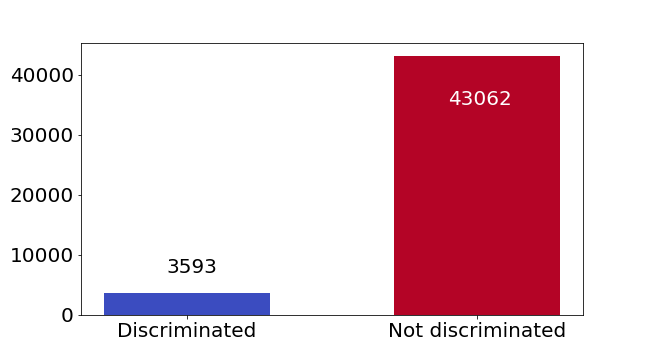
\includegraphics[width=0.48\textwidth]{../figures/tex/discriminated_small}
		\caption{Distribution of participants feeling discriminated against in their country.}
		\label{fig:discriminated_dist}
	\end{figure}
	
	If the question of feeling discriminated against was answered with "Yes", it was possible to select the specific form of discrimination from the following set of potential answers: color/race, nationality, religion, language, ethnic group, age, sexuality, disability, or other. 
	\begin{figure}[h]
		\centering
		\includegraphics[width=0.4\textwidth]{../figures/tex/discriminated_sub}
		\caption{Distribution of participants feeling discriminated against dependent on the reason.}
		\label{fig:discriminated_sub_dist}
	\end{figure}
	The overview of the chosen subcategories can be found in Figure \ref{fig:discriminated_sub_dist}. Since the subcategories of discrimination only contain less than 1000 data points each, it was not feasible to learn the type of discrimination specifically. Therefore, we focused only on the binary variable. 
	In order to understand the high numbers of people feeling discriminated against in specific countries (c.f. Figure \ref{fig:discriminated_country}), we investigated the subcategories of discrimination for these countries: The UK and France have a high percentage of people being discriminated based on color/race. In Iceland, discrimination based on age and gender are dominating while Montenegro leads the categories of discrimination based nationality and religion. 
	
	\subsection{Details of Data Preprocessing} \label{sec:details_preprocessing}
	As described in Section \ref{sec:data_set}, the options "Refusal", "Don't know", and "No answer" were included as outlier values, e.g. 7, 8, 9 for a question with the answers "Yes" (1) and "No"(0) in the data set. The gap between true answers and outliers increased significantly when large numerical values could be given as answers. This can be observed for the question "annual net pay" where the outliers are encoded with $7 \cdot 10^{9}, 8\cdot 10^{9}, 9 \cdot 10^{9}$. While some ML algorithms can deal with such distorted distributions, approaches like neural networks require benefit from a standardized and normalized input. Therefore, we decided to encode outliers dependent on the individual question. For a categorical scale with a center value, the outliers were mapped to this central value. If the scale had no such value, a center value was created artificially via shifting the upper part of the scale and assigning the outliers to the newly created center value. For numerical answers, the outliers were mapped to the median value.
	
	Furthermore, all data points containing NaN values were removed from the data set. This step reduced the number of samples from 49519 to 46655 and filtered out all data points corresponding to the countries Cyprus and Hungary.
	
	\begin{figure*}[t]
		\centering
		\includegraphics[width=\textwidth]{../figures/tex/decision_tree}
		\caption{Decision tree of model trained with feature set "all" and sampling method "non", displayed with a max\textunderscore depth $= 2$. For interpretation of the decision boundaries, please refer to the ESS documentation \cite{ESS9:2021}.}
		\label{fig:dt}
	\end{figure*}
	
	The variable indicating the country of a participant was encoded using one-hot encoding. Integer encoding is not suitable for this variable since putting the countries in a specific order has no intrinsic meaning and might only mislead the learning algorithm. Including the one-hot encoded country information, the total number of features is increased from 113 to 139.
	

	
	
	\subsection{Decision Tree} \label{ssec:dt}
	
	The visualized output of the decision tree models is useful to infer the importance of the features w.r.t. the target. Together with the results of the PCC calculations and the methods for explainability, expert knowledge from the field of the social sciences can be used to test or create assumptions on the dependencies of the features and the target.
	An example with a reduced depth to enable visualization is to be found in Figure \ref{fig:dt}. Additionally, a brief analysis of the paths resulting in the leaf nodes with respondents feeling discriminated against representing the majority class was performed. For the stated example, one of the paths resulting in a distribution of 35 non-discriminated and 73 discriminated training examples is associated with the following ordered decision rules: 
	
	\begin{enumerate}
		\item "Belong to minority ethnic group in country" <= 1.5,
		\item "Everyone in country fair chance achieve level of education they seek" <= 4.5,
		\item "Decisions in country politics are transparent" <= 2.5,
		\item "Confident in own ability to participate in politics" <= 3.5,
		\item "Mother's highest level of education" <= 162.5,
		\item "Most people try to take advantage of you, or try to be fair" <= 4.5 and
		\item "Take part in social activities compared to others of same age" <= 2.5.
	\end{enumerate}
	
\end{document}
